\subsection{Protocols}

	\par{The different building blocks of a network presented above allow for the transportation of information, but is is the use of protocols which provide the semantics. For a message to be decoded the parties involved must agree on some sort of well-defined syntax, so that noise can be separated from meaningul information, this is precisely the role of the various network protocols existing at all levels within a network.}

	\defn{PDU}{stands for protocol data unit, and is the basic unit	of information for any given protocol}

	\par{PDUs can be textual where rules of syntax and grammar are used to implement behaviour (e.g. HTTP), or binary where similar appropriate rules are used (e.g. TCP/IP). It is the role of PDUs to define what messages are legal to send, but is up to protocol semantics to define when to send them and what should be expected in response}

\subsubsection{Layers}

	\par{Communication systems are tipically organised into layers, which reduces complexity at each layer's level. Peers on the same layer, use that layer's protocol to communicate using services provided by the well-defined interfaces of the lower layers}

	\defn{OSI Model}{stands for \ita{Open Systems Interconnection Model} and is a conceptual model that characterises and standardises the communication functions of a telecommunication or computing system without regard to its underlying internal structure and technology. }

	\par{A design tool used widely to model layered communication channels is the \ita{OSI model}. It is merely a design tool, real implementations are more complex and usually the boundaries between layers are not so well defined.}

	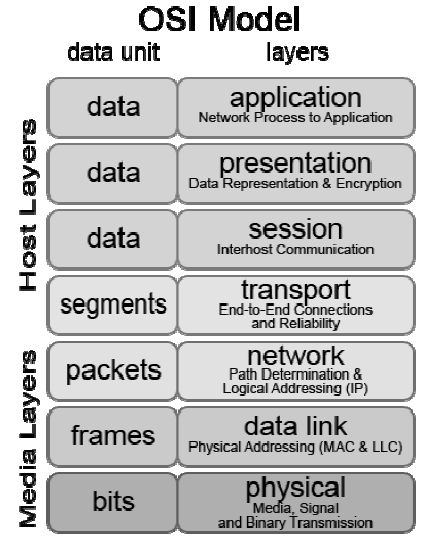
\includegraphics{osi.png}

\subsection{OSI - Physical Layer}

	\par{The physical layer is concernerd with the transmission of raw data bits. In order for this to be possbile, the information needs to be transformed and encoded and a decision on the best medium for the job (e.g. cables, fibre optic etc.) and their phyiscal properties needs to be taken.}

	\subsubsection{Transmission Channels - Enconding \& Modulation}

	\defn{Wired Data Trasmission}{ the signal is transmited over a cable and is \ita{directly} enconded onto the channel, by varying the voltage/light intensity}

	\defn{Wireless Data Transmssion}{ the signal is transmitted without the aid of an electrical conductor, most commonly using radio waves and some kind of modulation}

	\par{A signal can travel with or without the aid of an electrical condutor, if it is directly encoded into a cable, then one of several \ita{enconding schemes} can be used in order to change the signal into discrete pieces of data (e.g. bits).}

		\begin{itemize}
			\setlength\itemsep{0.5em}
			\mymarginpar{High $\approx [3,5]v$ , and Low $\approx [0,3)$}
			\mymarginpar{NRZ : Non-Return to Zero}
			\item\textbf{NRZ : }{1 -- High ; 0 -- Low}
			\item\textbf{NRZ Inverted : }{1 -- Change ; 0 -- Constant}
			\item\textbf{Manchester : }{1 -- High-Low ; 0 -- Low-High}
		\end{itemize}
		

		\todo{Insert image from anki card}

	\par{Alternatively one can encode information onto a channel by varying the properties of the carrier signal via a modulating signal, a process know as \ita{modulation} which allows the same channel to be shared by different signals}

		\todo{Insert image from anki card}

	\subsubsection{Bandwith, Capacity \& Noise}

	\defn{Bandwith}{ determines the frequency range it can transport}

	\defn{Sampling Theorem}{ states that to accurately digitise an analogue signal, $2H$ samples per second are needed, where $H$ is the bandwith in Hz}

	\defn{Signal-to-Noise Ratio}{ the ration between signal power and noise floor, typically quoten in dB $= 10\log(\frac{S}{N})$}

	\par{The bandwidth of a channel is determined by physicial limitations of the channel, and given the existence of noise in the real worl, the \ita{Signal-to-Noise} ratio and the bandwidth represent the fundamental limits for the rate at which information can be transmitted}

	\rem{The maximum transmission rate of a channel grows lograithmically to the SNR}

	\extra{Extra}{Theoretical Maximum Transmission Rate}{

		$$ R_{max} = 2H\log_{2}V $$

		where:
		\begin{itemize}
			\item[]$R_{max} =$ max trasmission rate in bits/s
			\item[]$H =$ bandwith in Hz
			\item[]$V =$ \# of discrete values per symbol
		\end{itemize}
	}

	\extra{Extra}{Shannon's Theorem}{
		$$ R_{max} = H\log_{2}(1 + SNR) $$

	}

	


	
	\subsubsection{Summary}

		\begin{itemize}
			\item\textbf{PDU : } bits
			\item\textbf{Function : } transmit a sequence of bits over an analogue channel
		\end{itemize} 
